\documentclass[11pt,compress,t,notes=noshow, xcolor=table]{beamer}
%<<setup-child, include = FALSE>>=
%library(knitr)
%library(qrmix)
%library(mlr)
%library(quantreg)
%library(reshape2)
%set_parent("../style/preamble.Rnw")
%@

% graphicx and color are loaded via lmu-lecture.sty
% maxwidth is the original width if it is less than linewidth
% otherwise use linewidth (to make sure the graphics do not exceed the margin)
% TODO: Remove once cleared to be superfluous
% \makeatletter
% \def\maxwidth{ %
%   \ifdim\Gin@nat@width>\linewidth
%     \linewidth
%   \else
%     \Gin@nat@width
%   \fi
% }
% \makeatother

% ---------------------------------%
% latex-math dependencies, do not remove:
% - mathtools
% - bm
% - siunitx
% - dsfont
% - xspace
% ---------------------------------%

%--------------------------------------------------------%
%       Language, encoding, typography
%--------------------------------------------------------%

\usepackage[english]{babel}
\usepackage[utf8]{inputenc} % Enables inputting UTF-8 symbols
% Standard AMS suite (loaded via lmu-lecture.sty)

% Font for double-stroke / blackboard letters for sets of numbers (N, R, ...)
% Distribution name is "doublestroke"
% According to https://mirror.physik.tu-berlin.de/pub/CTAN/fonts/doublestroke/dsdoc.pdf
% the "bbm" package does a similar thing and may be superfluous.
% Required for latex-math
\usepackage{dsfont}

% bbm – "Blackboard-style" cm fonts (https://www.ctan.org/pkg/bbm)
% Used to be in common.tex, loaded directly after this file
% Maybe superfluous given dsfont is loaded
% TODO: Check if really unused?
% \usepackage{bbm}

% bm – Access bold symbols in maths mode - https://ctan.org/pkg/bm
% Required for latex-math, preferred over \boldsymbol
% https://tex.stackexchange.com/questions/3238/bm-package-versus-boldsymbol
\usepackage{bm}

% pifont – Access to PostScript standard Symbol and Dingbats fonts
% Used for \newcommand{\xmark}{\ding{55}, which is never used
% aside from lecture_advml/attic/xx-automl/slides.Rnw
% \usepackage{pifont}

% Quotes (inline and display), provdes \enquote
% https://ctan.org/pkg/csquotes
\usepackage{csquotes}

% Adds arg to enumerate env, technically superseded by enumitem according
% to https://ctan.org/pkg/enumerate
% Replace with https://ctan.org/pkg/enumitem ?
% Even better: enumitem is not really compatible with beamer and breaks all sorts of things
% particularly the enumerate environment. The enumerate package also just isn't required
% from what I can tell so... don't re-add it I guess?
% \usepackage{enumerate}

% Line spacing - provides \singlespacing \doublespacing \onehalfspacing
% https://ctan.org/pkg/setspace
% \usepackage{setspace}

% mathtools – Mathematical tools to use with amsmath
% https://ctan.org/pkg/mathtools?lang=en
% latex-math dependency according to latex-math repo
\usepackage{mathtools}

% Maybe not great to use this https://tex.stackexchange.com/a/197/19093
% Use align instead -- TODO: Global search & replace to check, eqnarray is used a lot
% $ rg -f -u "\begin{eqnarray" -l | grep -v attic | awk -F '/' '{print $1}' | sort | uniq -c
%   13 lecture_advml
%   14 lecture_i2ml
%    2 lecture_iml
%   27 lecture_optimization
%   45 lecture_sl
\usepackage{eqnarray}
% For shaded regions / boxes
% Used sometimes in optim
% https://www.ctan.org/pkg/framed
\usepackage{framed}

%--------------------------------------------------------%
%       Cite button (version 2024-05)
%--------------------------------------------------------%

% Superseded by style/ref-buttons.sty, kept just in case these don't work out somehow.

% Note this requires biber to be in $PATH when running,
% telltale error in log would be e.g. Package biblatex Info: ... file 'authoryear.dbx' not found
% aside from obvious "biber: command not found" or similar.
% Tried moving this to lmu-lecture.sty but had issues I didn't quite understood,
% so it's here for now.

\usepackage{hyperref}

% Only try adding a references file if it exists, otherwise
% this would compile error when references.bib is not found
% NOTE: Bibliography packages (usebib, biblatex) are now loaded by ref-buttons.sty when needed
% This keeps all bibliography-related setup in one place

% Legacy \citelink command removed - superseded by ref-buttons.sty

%--------------------------------------------------------%
%       Displaying code and algorithms
%--------------------------------------------------------%

% Reimplements verbatim environments: https://ctan.org/pkg/verbatim
% verbatim used sed at least once in
% supervised-classification/slides-classification-tasks.tex
% Removed since code should not be put on slides anyway
% \usepackage{verbatim}

% Both used together for algorithm typesetting, see also overleaf: https://www.overleaf.com/learn/latex/Algorithms
% algorithmic env is also used, but part of the bundle:
%   "algpseudocode is part of the algorithmicx bundle, it gives you an improved version of algorithmic besides providing some other features"
% According to https://tex.stackexchange.com/questions/229355/algorithm-algorithmic-algorithmicx-algorithm2e-algpseudocode-confused
\usepackage{algorithm}
\usepackage{algpseudocode}

%--------------------------------------------------------%
%       Tables
%--------------------------------------------------------%

% multi-row table cells: https://www.namsu.de/Extra/pakete/Multirow.html
% Provides \multirow
% Used e.g. in evaluation/slides-evaluation-measures-classification.tex
\usepackage{multirow}

% colortbl: https://ctan.org/pkg/colortbl
% "The package allows rows and columns to be coloured, and even individual cells." well.
% Provides \columncolor and \rowcolor
% \rowcolor is used multiple times, e.g. in knn/slides-knn.tex
\usepackage{colortbl}

% long/multi-page tables: https://texdoc.org/serve/longtable.pdf/0
% Not used in slides
% \usepackage{longtable}

% pretty table env: https://ctan.org/pkg/booktabs
% Is used
% Defines \toprule
\usepackage{booktabs}

%--------------------------------------------------------%
%       Figures: Creating, placing, verbing
%--------------------------------------------------------%

% wrapfig - Wrapping text around figures https://de.overleaf.com/learn/latex/Wrapping_text_around_figures
% Provides wrapfigure environment -used in lecture_optimization
\usepackage{wrapfig}

% Sub figures in figures and tables
% https://ctan.org/pkg/subfig -- supersedes subfigure package
% Provides \subfigure
% \subfigure not used in slides but slides-tuning-practical.pdf errors without this pkg, error due to \captionsetup undefined
\usepackage{subfig}

% Actually it's pronounced PGF https://en.wikibooks.org/wiki/LaTeX/PGF/TikZ
\usepackage{tikz}

% No idea what/why these settings are what they are but I assume they're there on purpose
\usetikzlibrary{shapes,arrows,automata,positioning,calc,chains,trees, shadows}
\tikzset{
  %Define standard arrow tip
  >=stealth',
  %Define style for boxes
  punkt/.style={
    rectangle,
    rounded corners,
    draw=black, very thick,
    text width=6.5em,
    minimum height=2em,
    text centered},
  % Define arrow style
  pil/.style={
    ->,
    thick,
    shorten <=2pt,
    shorten >=2pt,}
}

%--------------------------------------------------------%
%       Beamer setup and custom macros & environments
%--------------------------------------------------------%

% Main sty file for beamer setup (layout, style, lecture page numbering, etc.)
% For long-term maintenance, this may me refactored into a more modular set of .sty files
\usepackage{../../style/lmu-lecture}
% Custom itemize wrappers, itemizeS, itemizeL, etc
\usepackage{../../style/customitemize}
% Custom framei environment, uses custom itemize!
\usepackage{../../style/framei}
% Custom frame2 environment, allows specifying font size for all content
\usepackage{../../style/frame2}
% Column layout macros
\usepackage{../../style/splitV}
% \image and derivatives
\usepackage{../../style/image}
% New generation of reference button macros
\usepackage{../../style/ref-buttons}

% Used regularly
\let\code=\texttt

% Not sure what/why this does
\setkeys{Gin}{width=0.9\textwidth}

% -- knitr leftovers --
% These may be used by knitr/R Markdown workflows in other lectures
\makeatletter
\def\maxwidth{ %
  \ifdim\Gin@nat@width>\linewidth
    \linewidth
  \else
    \Gin@nat@width
  \fi
}
\makeatother

% Define colors for syntax highlighting (may be used by knitr)
\definecolor{fgcolor}{rgb}{0.345, 0.345, 0.345}
\definecolor{shadecolor}{rgb}{.97, .97, .97}

% knitr code output environment
\newenvironment{knitrout}{}{}


% Can't find a reason why common.tex is not just part of this file?
\input{../../style/common}

\input{../../latex-math/basic-math}
% machine learning
\newcommand{\Xspace}{\mathcal{X}} % X, input space
\newcommand{\Yspace}{\mathcal{Y}} % Y, output space
\newcommand{\Zspace}{\mathcal{Z}} % Z, space of sampled datapoints
\newcommand{\nset}{\{1, \ldots, n\}} % set from 1 to n
\newcommand{\pset}{\{1, \ldots, p\}} % set from 1 to p
\newcommand{\gset}{\{1, \ldots, g\}} % set from 1 to g
\newcommand{\Pxy}{\mathbb{P}_{xy}} % P_xy
\newcommand{\Exy}{\mathbb{E}_{xy}} % E_xy: Expectation over random variables xy
\newcommand{\xv}{\mathbf{x}} % vector x (bold)
\newcommand{\xtil}{\tilde{\mathbf{x}}} % vector x-tilde (bold)
\newcommand{\yv}{\mathbf{y}} % vector y (bold)
\newcommand{\xy}{(\xv, y)} % observation (x, y)
\newcommand{\xvec}{\left(x_1, \ldots, x_p\right)^\top} % (x1, ..., xp)
\newcommand{\Xmat}{\mathbf{X}} % Design matrix
\newcommand{\allDatasets}{\mathds{D}} % The set of all datasets
\newcommand{\allDatasetsn}{\mathds{D}_n}  % The set of all datasets of size n
\newcommand{\D}{\mathcal{D}} % D, data
\newcommand{\Dn}{\D_n} % D_n, data of size n
\newcommand{\Dtrain}{\mathcal{D}_{\text{train}}} % D_train, training set
\newcommand{\Dtest}{\mathcal{D}_{\text{test}}} % D_test, test set
\newcommand{\xyi}[1][i]{\left(\xv^{(#1)}, y^{(#1)}\right)} % (x^i, y^i), i-th observation
\newcommand{\Dset}{\left( \xyi[1], \ldots, \xyi[n]\right)} % {(x1,y1)), ..., (xn,yn)}, data
\newcommand{\defAllDatasetsn}{(\Xspace \times \Yspace)^n} % Def. of the set of all datasets of size n
\newcommand{\defAllDatasets}{\bigcup_{n \in \N}(\Xspace \times \Yspace)^n} % Def. of the set of all datasets
\newcommand{\xdat}{\left\{ \xv^{(1)}, \ldots, \xv^{(n)}\right\}} % {x1, ..., xn}, input data
\newcommand{\ydat}{\left\{ \yv^{(1)}, \ldots, \yv^{(n)}\right\}} % {y1, ..., yn}, input data
\newcommand{\yvec}{\left(y^{(1)}, \hdots, y^{(n)}\right)^\top} % (y1, ..., yn), vector of outcomes
\newcommand{\greekxi}{\xi} % Greek letter xi
\renewcommand{\xi}[1][i]{\xv^{(#1)}} % x^i, i-th observed value of x
\newcommand{\yi}[1][i]{y^{(#1)}} % y^i, i-th observed value of y
\newcommand{\xivec}{\left(x^{(i)}_1, \ldots, x^{(i)}_p\right)^\top} % (x1^i, ..., xp^i), i-th observation vector
\newcommand{\xj}{\xv_j} % x_j, j-th feature
\newcommand{\xjvec}{\left(x^{(1)}_j, \ldots, x^{(n)}_j\right)^\top} % (x^1_j, ..., x^n_j), j-th feature vector
\newcommand{\phiv}{\mathbf{\phi}} % Basis transformation function phi
\newcommand{\phixi}{\mathbf{\phi}^{(i)}} % Basis transformation of xi: phi^i := phi(xi)

%%%%%% ml - models general
\newcommand{\lamv}{\bm{\lambda}} % lambda vector, hyperconfiguration vector
\newcommand{\Lam}{\Lambda}	 % Lambda, space of all hpos
% Inducer / Inducing algorithm
\newcommand{\preimageInducer}{\left(\defAllDatasets\right)\times\Lam} % Set of all datasets times the hyperparameter space
\newcommand{\preimageInducerShort}{\allDatasets\times\Lam} % Set of all datasets times the hyperparameter space
% Inducer / Inducing algorithm
\newcommand{\ind}{\mathcal{I}} % Inducer, inducing algorithm, learning algorithm

% continuous prediction function f
\newcommand{\ftrue}{f_{\text{true}}}  % True underlying function (if a statistical model is assumed)
\newcommand{\ftruex}{\ftrue(\xv)} % True underlying function (if a statistical model is assumed)
\newcommand{\fx}{f(\xv)} % f(x), continuous prediction function
\newcommand{\fdomains}{f: \Xspace \rightarrow \R^g} % f with domain and co-domain
\newcommand{\Hspace}{\mathcal{H}} % hypothesis space where f is from
\newcommand{\Hall}{\mathcal{H}_{\text{all}}} % unrestricted hypothesis space
\newcommand{\fbayes}{f^{\ast}} % Bayes-optimal model
\newcommand{\fxbayes}{f^{\ast}(\xv)} % Bayes-optimal model
\newcommand{\fkx}[1][k]{f_{#1}(\xv)} % f_j(x), discriminant component function
\newcommand{\fhspace}{\hat f_{\Hspace}} % fhat_H
\newcommand{\fh}{\hat{f}} % f hat, estimated prediction function
\newcommand{\fxh}{\fh(\xv)} % fhat(x)
\newcommand{\fxt}{f(\xv ~|~ \thetav)} % f(x | theta)
\newcommand{\fxi}{f\left(\xv^{(i)}\right)} % f(x^(i))
\newcommand{\fxih}{\hat{f}\left(\xv^{(i)}\right)} % f(x^(i))
\newcommand{\fxit}{f\big(\xv^{(i)} ~|~ \thetav\big)} % f(x^(i) | theta)
\newcommand{\fhD}{\fh_{\D}} % fhat_D, estimate of f based on D
\newcommand{\fhDtrain}{\fh_{\Dtrain}} % fhat_Dtrain, estimate of f based on D
\newcommand{\fhDnlam}{\fh_{\Dn, \lamv}} %model learned on Dn with hp lambda
\newcommand{\fhDlam}{\fh_{\D, \lamv}} %model learned on D with hp lambda
\newcommand{\fhDnlams}{\fh_{\Dn, \lamv^\ast}} %model learned on Dn with optimal hp lambda
\newcommand{\fhDlams}{\fh_{\D, \lamv^\ast}} %model learned on D with optimal hp lambda

% discrete prediction function h
\newcommand{\hx}{h(\xv)} % h(x), discrete prediction function
\newcommand{\hh}{\hat{h}} % h hat
\newcommand{\hxh}{\hat{h}(\xv)} % hhat(x)
\newcommand{\hxt}{h(\xv | \thetav)} % h(x | theta)
\newcommand{\hxi}{h\left(\xi\right)} % h(x^(i))
\newcommand{\hxit}{h\left(\xi ~|~ \thetav\right)} % h(x^(i) | theta)
\newcommand{\hbayes}{h^{\ast}} % Bayes-optimal classification model
\newcommand{\hxbayes}{h^{\ast}(\xv)} % Bayes-optimal classification model

% yhat
\newcommand{\yh}{\hat{y}} % yhat for prediction of target
\newcommand{\yih}{\hat{y}^{(i)}} % yhat^(i) for prediction of ith targiet
\newcommand{\resi}{\yi- \yih}

% theta
\newcommand{\thetah}{\hat{\theta}} % theta hat
\newcommand{\thetav}{\bm{\theta}} % theta vector
\newcommand{\thetavh}{\bm{\hat\theta}} % theta vector hat
\newcommand{\thetat}[1][t]{\thetav^{[#1]}} % theta^[t] in optimization
\newcommand{\thetatn}[1][t]{\thetav^{[#1 +1]}} % theta^[t+1] in optimization
\newcommand{\thetahDnlam}{\thetavh_{\Dn, \lamv}} %theta learned on Dn with hp lambda
\newcommand{\thetahDlam}{\thetavh_{\D, \lamv}} %theta learned on D with hp lambda
\newcommand{\mint}{\min_{\thetav \in \Theta}} % min problem theta
\newcommand{\argmint}{\argmin_{\thetav \in \Theta}} % argmin theta

% densities + probabilities
% pdf of x
\newcommand{\pdf}{p} % p
\newcommand{\pdfx}{p(\xv)} % p(x)
\newcommand{\pixt}{\pi(\xv~|~ \thetav)} % pi(x|theta), pdf of x given theta
\newcommand{\pixit}[1][i]{\pi\left(\xi[#1] ~|~ \thetav\right)} % pi(x^i|theta), pdf of x given theta
\newcommand{\pixii}[1][i]{\pi\left(\xi[#1]\right)} % pi(x^i), pdf of i-th x

% pdf of (x, y)
\newcommand{\pdfxy}{p(\xv,y)} % p(x, y)
\newcommand{\pdfxyt}{p(\xv, y ~|~ \thetav)} % p(x, y | theta)
\newcommand{\pdfxyit}{p\left(\xi, \yi ~|~ \thetav\right)} % p(x^(i), y^(i) | theta)

% pdf of x given y
\newcommand{\pdfxyk}[1][k]{p(\xv | y= #1)} % p(x | y = k)
\newcommand{\lpdfxyk}[1][k]{\log p(\xv | y= #1)} % log p(x | y = k)
\newcommand{\pdfxiyk}[1][k]{p\left(\xi | y= #1 \right)} % p(x^i | y = k)

% prior probabilities
\newcommand{\pik}[1][k]{\pi_{#1}} % pi_k, prior
\newcommand{\pih}{\hat{\pi}} % pi hat, estimated prior (binary classification)
\newcommand{\pikh}[1][k]{\hat{\pi}_{#1}} % pi_k hat, estimated prior
\newcommand{\lpik}[1][k]{\log \pi_{#1}} % log pi_k, log of the prior
\newcommand{\pit}{\pi(\thetav)} % Prior probability of parameter theta

% posterior probabilities
\newcommand{\post}{\P(y = 1 ~|~ \xv)} % P(y = 1 | x), post. prob for y=1
\newcommand{\postk}[1][k]{\P(y = #1 ~|~ \xv)} % P(y = k | y), post. prob for y=k
\newcommand{\pidomains}{\pi: \Xspace \rightarrow \unitint} % pi with domain and co-domain
\newcommand{\pibayes}{\pi^{\ast}} % Bayes-optimal classification model
\newcommand{\pixbayes}{\pi^{\ast}(\xv)} % Bayes-optimal classification model
\newcommand{\piastxtil}{\pi^{\ast}(\xtil)} % Bayes-optimal classification model
\newcommand{\piastkxtil}{\pi^{\ast}_k(\xtil)} % Bayes-optimal classification model for k-th class
\newcommand{\pix}{\pi(\xv)} % pi(x), P(y = 1 | x)
\newcommand{\piv}{\bm{\pi}} % pi, bold, as vector
\newcommand{\pikx}[1][k]{\pi_{#1}(\xv)} % pi_k(x), P(y = k | x)
\newcommand{\pikxt}[1][k]{\pi_{#1}(\xv ~|~ \thetav)} % pi_k(x | theta), P(y = k | x, theta)
\newcommand{\pixh}{\hat \pi(\xv)} % pi(x) hat, P(y = 1 | x) hat
\newcommand{\pikxh}[1][k]{\hat \pi_{#1}(\xv)} % pi_k(x) hat, P(y = k | x) hat
\newcommand{\pixih}{\hat \pi(\xi)} % pi(x^(i)) with hat
\newcommand{\pikxih}[1][k]{\hat \pi_{#1}(\xi)} % pi_k(x^(i)) with hat
\newcommand{\pdfygxt}{p(y ~|~\xv, \thetav)} % p(y | x, theta)
\newcommand{\pdfyigxit}{p\left(\yi ~|~\xi, \thetav\right)} % p(y^i |x^i, theta)
\newcommand{\lpdfygxt}{\log \pdfygxt } % log p(y | x, theta)
\newcommand{\lpdfyigxit}{\log \pdfyigxit} % log p(y^i |x^i, theta)

% probabilistic
\newcommand{\bayesrulek}[1][k]{\frac{\P(\xv | y= #1) \P(y= #1)}{\P(\xv)}} % Bayes rule
\newcommand{\muv}{\bm{\mu}} % expectation vector of Gaussian
\newcommand{\muk}[1][k]{\bm{\mu_{#1}}} % mean vector of class-k Gaussian (discr analysis)
\newcommand{\mukh}[1][k]{\bm{\hat{\mu}_{#1}}} % estimated mean vector of class-k Gaussian (discr analysis)

% residual and margin
\newcommand{\rx}{r(\xv)} % residual 
\newcommand{\eps}{\epsilon} % residual, stochastic
\newcommand{\epsv}{\bm{\epsilon}} % residual, stochastic, as vector
\newcommand{\epsi}{\epsilon^{(i)}} % epsilon^i, residual, stochastic
\newcommand{\epsh}{\hat{\epsilon}} % residual, estimated
\newcommand{\epsvh}{\hat{\epsv}} % residual, estimated, vector
\newcommand{\yf}{y \fx} % y f(x), margin
\newcommand{\yfi}{\yi \fxi} % y^i f(x^i), margin
\newcommand{\Sigmah}{\hat \Sigma} % estimated covariance matrix
\newcommand{\Sigmahj}{\hat \Sigma_j} % estimated covariance matrix for the j-th class
\newcommand{\nux}{\nu(\xv)} % nu(x) = y * f(x)

% ml - loss, risk, likelihood
\newcommand{\Lyf}{L\left(y, f\right)} % L(y, f), loss function
% \newcommand{\Lypi}{L\left(y, \pi\right)} % L(y, pi), loss function
\newcommand{\Lxy}{L\left(y, \fx\right)} % L(y, f(x)), loss function
\newcommand{\Lxyi}{L\left(\yi, \fxi\right)} % loss of observation
\newcommand{\Lxyt}{L\left(y, \fxt\right)} % loss with f parameterized
\newcommand{\Lxyit}{L\left(\yi, \fxit\right)} % loss of observation with f parameterized
\newcommand{\Lxym}{L\left(\yi, f\left(\bm{\tilde{x}}^{(i)} ~|~ \thetav\right)\right)} % loss of observation with f parameterized
\newcommand{\Lpixy}{L\left(y, \pix\right)} % loss in classification
% \newcommand{\Lpiy}{L\left(y, \pi\right)} % loss in classification
\newcommand{\Lpiv}{L\left(y, \piv\right)} % loss in classification
\newcommand{\Lpixyi}{L\left(\yi, \pixii\right)} % loss of observation in classification
\newcommand{\Lpixyt}{L\left(y, \pixt\right)} % loss with pi parameterized
\newcommand{\Lpixyit}{L\left(\yi, \pixit\right)} % loss of observation with pi parameterized
% \newcommand{\Lhy}{L\left(y, h\right)} % L(y, h), loss function on discrete classes
\newcommand{\Lhxy}{L\left(y, \hx\right)} % L(y, h(x)), loss function on discrete classes
\newcommand{\Lr}{L\left(r\right)} % L(r), loss defined on residual (reg) / margin (classif)
\newcommand{\lone}{|y - \fx|} % L1 loss
\newcommand{\ltwo}{\left(y - \fx\right)^2} % L2 loss
\newcommand{\lbernoullimp}{\ln(1 + \exp(-y \cdot \fx))} % Bernoulli loss for -1, +1 encoding
\newcommand{\lbernoullizo}{- y \cdot \fx + \log(1 + \exp(\fx))} % Bernoulli loss for 0, 1 encoding
\newcommand{\lcrossent}{- y \log \left(\pix\right) - (1 - y) \log \left(1 - \pix\right)} % cross-entropy loss
\newcommand{\lbrier}{\left(\pix - y \right)^2} % Brier score
\newcommand{\risk}{\mathcal{R}} % R, risk
\newcommand{\riskbayes}{\mathcal{R}^\ast}
\newcommand{\riskf}{\risk(f)} % R(f), risk
\newcommand{\riskdef}{\E_{y|\xv}\left(\Lxy \right)} % risk def (expected loss)
\newcommand{\riskt}{\mathcal{R}(\thetav)} % R(theta), risk
\newcommand{\riske}{\mathcal{R}_{\text{emp}}} % R_emp, empirical risk w/o factor 1 / n
\newcommand{\riskeb}{\bar{\mathcal{R}}_{\text{emp}}} % R_emp, empirical risk w/ factor 1 / n
\newcommand{\riskef}{\riske(f)} % R_emp(f)
\newcommand{\risket}{\mathcal{R}_{\text{emp}}(\thetav)} % R_emp(theta)
\newcommand{\riskr}{\mathcal{R}_{\text{reg}}} % R_reg, regularized risk
\newcommand{\riskrt}{\mathcal{R}_{\text{reg}}(\thetav)} % R_reg(theta)
\newcommand{\riskrf}{\riskr(f)} % R_reg(f)
\newcommand{\riskrth}{\hat{\mathcal{R}}_{\text{reg}}(\thetav)} % hat R_reg(theta)
\newcommand{\risketh}{\hat{\mathcal{R}}_{\text{emp}}(\thetav)} % hat R_emp(theta)
\newcommand{\LL}{\mathcal{L}} % L, likelihood
\newcommand{\LLt}{\mathcal{L}(\thetav)} % L(theta), likelihood
\newcommand{\LLtx}{\mathcal{L}(\thetav | \xv)} % L(theta|x), likelihood
\newcommand{\logl}{\ell} % l, log-likelihood
\newcommand{\loglt}{\logl(\thetav)} % l(theta), log-likelihood
\newcommand{\logltx}{\logl(\thetav | \xv)} % l(theta|x), log-likelihood
\newcommand{\errtrain}{\text{err}_{\text{train}}} % training error
\newcommand{\errtest}{\text{err}_{\text{test}}} % test error
\newcommand{\errexp}{\overline{\text{err}_{\text{test}}}} % avg training error

% lm
\newcommand{\thx}{\thetav^\top \xv} % linear model
\newcommand{\olsest}{(\Xmat^\top \Xmat)^{-1} \Xmat^\top \yv} % OLS estimator in LM


\title{Introduction to Machine Learning}

\begin{document}
    
\titlemeta{% Chunk title (example: CART, Forests, Boosting, ...), can be empty
    Advanced Risk Minimization
  }{% Lecture title  
    Maximum Likelihood Estimation vs.
    Empirical Risk Minimization
  }{% Relative path to title page image: Can be empty but must not start with slides/
  figure/residuals_plot_L1_title.png
  }{
  \item Correspondence between Laplace errors and L1 loss
	\item Correspondence between Bernoulli targets and the Bernoulli / log loss 
}

\begin{vbframe}{Laplace Errors - L1-Loss}

Let's consider Laplacian errors $\eps$ now, with density: 

\begin{minipage}{0.5\textwidth}
$$
 \frac{1}{2\sigma} \exp\left(-\frac{|\eps|}{\sigma}\right)\,, \sigma > 0.
$$
\end{minipage}%
\begin{minipage}{0.5\textwidth}
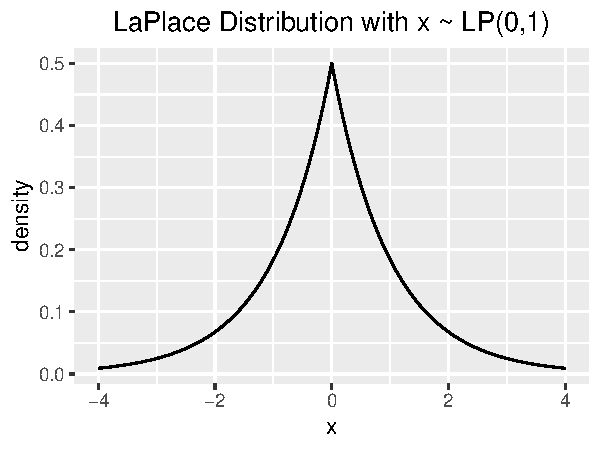
\includegraphics[width = 0.75\textwidth]{figure/laplace_plot.pdf}
\end{minipage}
Then
$$
y = \ftrue(\xv) + \eps 
$$

also follows Laplace distrib. with mean $\fxit$ and scale  $\sigma$. 

\framebreak 

The likelihood is then 

\begin{eqnarray*}
\LL(\thetab) &=& \prod_{i=1}^n \pdf\left(\yi ~\bigg|~ \fxit, \sigma\right) \\ &\propto& \exp\left(-\frac{1}{\sigma}\sumin \left|\yi - \fxit\right|\right)\,.
\end{eqnarray*}
The negative log-likelihood is
$$
- \loglt \propto \sumin \left|\yi - \fxit\right|.
$$

MLE for Laplacian errors = ERM with L1-loss. 

\begin{itemize}
\item Some losses correspond to more complex or less known error densities, like the Huber loss \citelink{meyer2021alternative}

\item Huber density is (unsurprisingly) a hybrid of Gaussian and Laplace

\end{itemize}

\framebreak 

\begin{footnotesize}
\begin{itemize}
	\item We simulate data $y ~|~\xv \sim \text{Laplacian}\left(\ftrue(\xv), 1\right)$ with $\ftrue = 0.2 \cdot \xv$. 
\item We can plot the empirical error distribution, i.e. the distribution of the residuals after fitting a regression model w.r.t. $L1$-loss.
\item With the help of a Q-Q-plot we can compare the empirical residuals vs. the theoretical quantiles of a Laplacian distribution.  
\end{itemize}
\end{footnotesize}
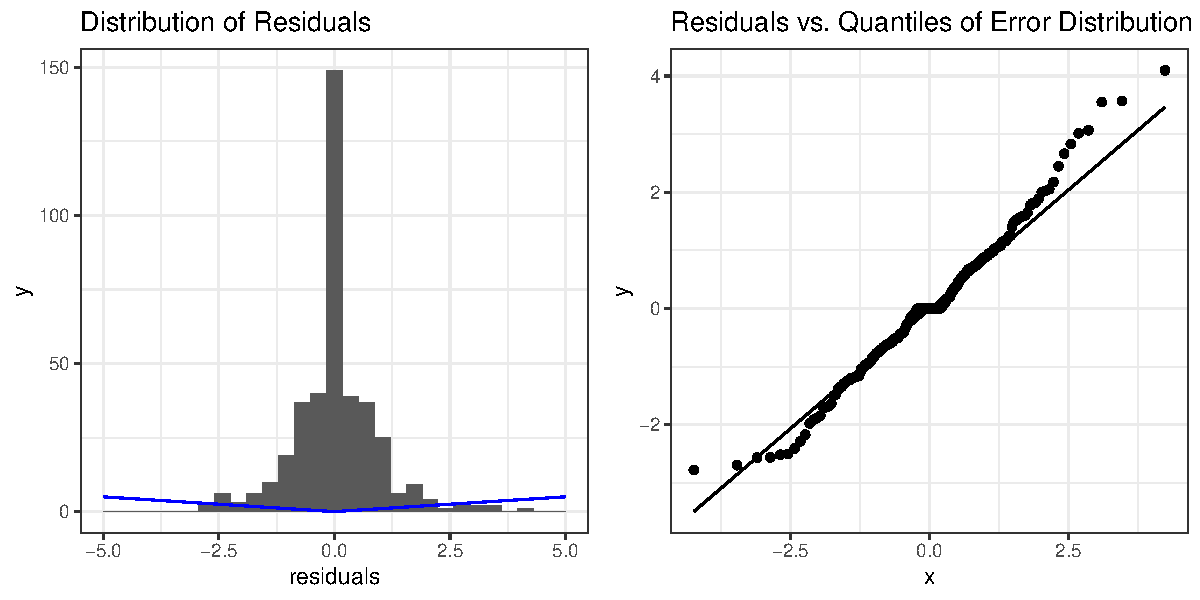
\includegraphics{figure/residuals_plot_L1.pdf}



\end{vbframe}



\begin{vbframe}{Maximum Likelihood in Classification}

Let us assume the outputs $y$ to be Bernoulli-distributed, i.e.  

$$
  y ~|~ \xv \sim \text{Ber}(\pi_\text{true}(\xv)). 
$$

The negative log likelihood is

\begin{eqnarray*}
- \loglt &=& -\sumin \lpdfyigxit \\ 
&=& - \sumin \log \left[\pi\left(\xi\right)^{y^{(i)}} \cdot \left(1 - \pi\left(\xi\right)\right)^{(1 - y^{(i)})} \right]\\
&=& \sumin -\yi \log[\pi\left(\xi\right)] - \left(1-\yi\right) \log [1 - \pi\left(\xi\right)]. 
\end{eqnarray*}


\framebreak 

This gives rise to the following loss function 

$$
  L(y, \pix) = -y\log(\pix)-(1-y)\log(1-\pix), \quad y \in \{0, 1\}
$$

which we introduced as \textbf{Bernoulli} loss. 

\vspace{0.2cm}

\begin{center}
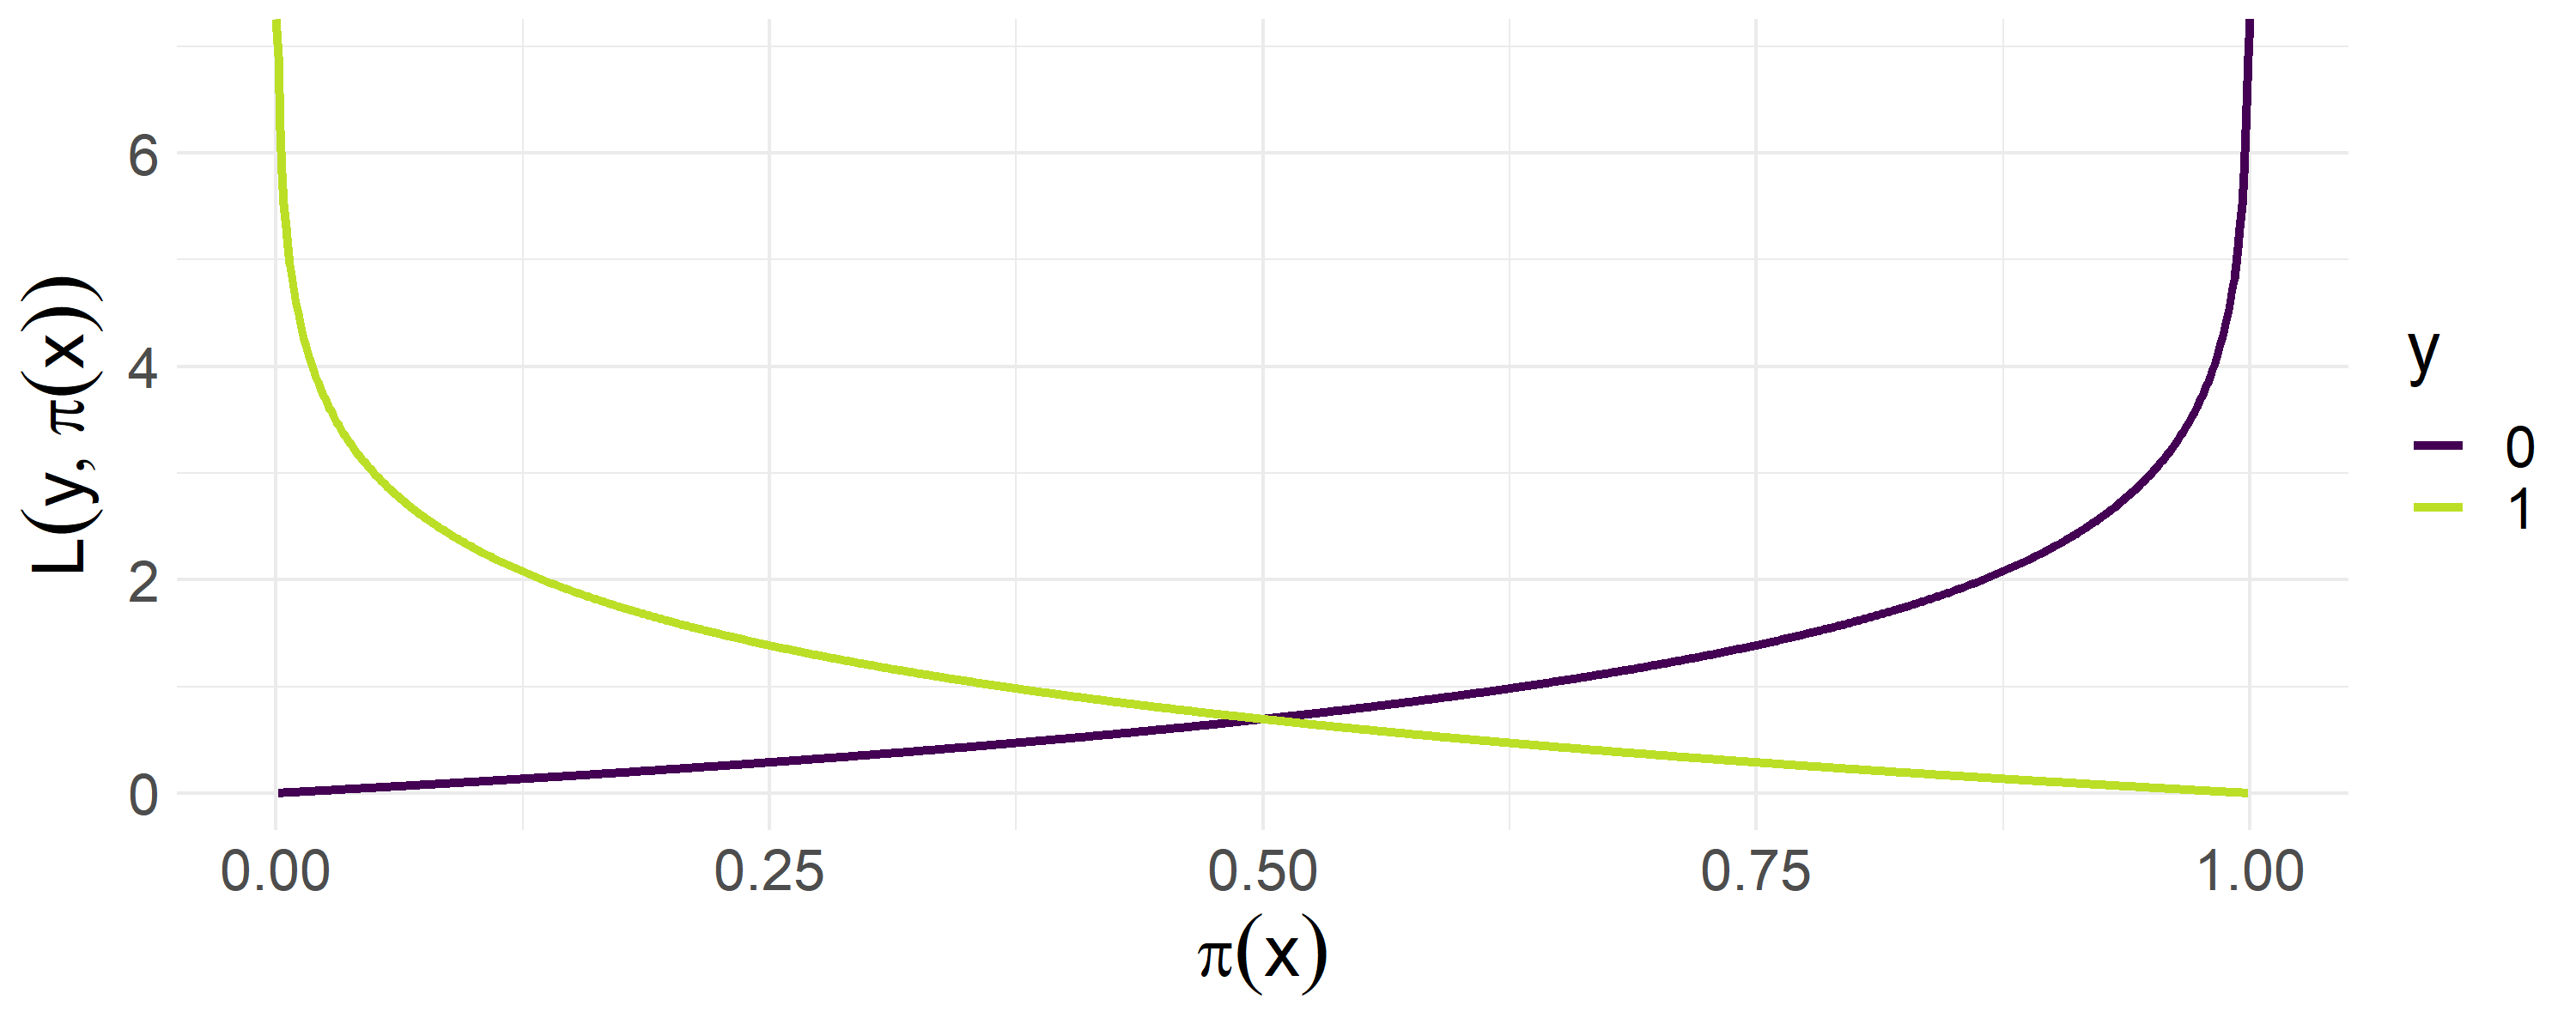
\includegraphics[width = 11cm ]{figure/plot_bernoulli_prob.png} \\
\end{center}



% \framebreak 

% The Bernoulli loss is used in \textbf{logistic regression} in combination with the hypothesis space of linear functions

% \vspace*{-0.3cm}

% \begin{eqnarray*}
%   \Hspace = \left\{f: \Xspace \to \R ~|~\fx = \thetab^\top \xv\right\}
% \end{eqnarray*}

% Scores are afterwards transformed into probabilities by the logistic function $\pix = \left(1 + \exp(- \fx)\right)^{-1}$  

% \begin{center}
%   \includegraphics[width = 0.4\textwidth]{figure_man/logreg-2vars-data.png}~~\includegraphics[width = 0.4\textwidth]{figure_man/logreg-2vars-score-vs-prob.png}
% \end{center}

% \framebreak

% \begin{center}
%   \includegraphics[width=0.8\textwidth]{figure_man/logreg-2vars-surface.png}
% \end{center}


\end{vbframe}




% \begin{vbframe}{Classification Losses: Bernoulli Loss}
% \begin{itemize}
%   \item $L(y, \pix) = -y\ln(\pix)-(1-y)\ln(1-\pix) $
%   % \item Also called \textbf{Bernoulli Loss}
%   \item Convex, differentiable (gradient methods can be used), not robust
%   \item Also called logarithmic loss or cross-entropy loss (which will be motivated later)
% \end{itemize}


% \framebreak 

% \lz 

% The constant model $\pix =< \theta$ that is optimal w.r.t. the empirical risk is the fraction of class $1$ observations

% $$
% \hat \pi (\xv) = \frac{1}{n}\sumin \yi.
% $$

% \textbf{Proof:} Exercise.


% \end{vbframe}



% \begin{vbframe}{Classification Losses: Cross-Entropy Loss}

% \begin{itemize}
%   \item The cross entropy loss 
%   $$
%   \Lxy = -y\ln(\pix)-(1-y)\ln(1-\pix)$$
%   % is equivalent to logistic loss when 
%   \item  The cross entropy loss is closely related to the Kullback-Leibler divergence, which will be introduced later in the chapter.
%   \item Very often used in neural networks with binary output nodes for classification.
% \end{itemize}

% \end{vbframe}

% \section{Outlook}

% \begin{vbframe}{Outlook}

% When introducing different learning algorithms, we will come back to the loss functions introduced in this chapter or even introduce new ones. For example:  

% \begin{itemize}
%   \item Ordinary Linear Regression: L2-loss
%   \item Logistic Regression: Logistic loss
%   \item Support Vector Machine Classification: Hinge-Loss (to be introduced) (see \textbf{SVM} chapter)
%   \item Support Vector Machine Regression: $\epsilon$-insensitive loss (see \textbf{SVM} chapter)
%   \item AdaBoost: Exponential loss (see \textbf{Boosting} chapter)
% \end{itemize}

% Once knowing the theory of risk minimization and properties of loss functions, we can combine model classes and loss functions as needed or even tailor loss functions to our needs. 

% \end{vbframe}

% \framebreak

% we get the risk function

% \begin{eqnarray*}
% \risk(f) &=& \mathbb{E}_x [\max\{0, 1 - \fx\} \pix + \max\{0, 1 + y\fx\} (1-\pix)].
% \end{eqnarray*}

% The minimizer of $\risk(f)$ for the hinge loss function is

% \begin{eqnarray*}
  % $fh(x) =  \footnotesize \begin{cases} 1 \quad \text{ if } \pix > 1/2 \\ -1 \quad \pix < 1/2  \end{cases}$
% \end{eqnarray*}



% \section{Selected methods for regression and classification}

% \begin{vbframe}{Normal linear and additive regression}

% For $i \in \nset$ (simple case and with basis functions):
% \begin{eqnarray*}
% \yi & = & \fxi + \epsi = \theta_0 + \theta^T \xi + \epsi\\
% \yi & = & \fxi + \epsi = \theta_0 + \theta^T \phi(\xi) + \epsi
% \end{eqnarray*}

% \begin{itemize}
% \item basis functions $\phi(x)=(\phi_1(x), \ldots, \phi_m(x))^T$
% \item assumption: $\epsi \iid N(0, \sigma^2)$
% \end{itemize}

% \lz

% Given observed data $\D$  we want to address the questions
% \begin{itemize}
% \item  Given basis functions, how to find $\theta$? ({\bf Parameter estimation})
% \item  How to select basis functions for my problem? ({\bf Model selection} )
% \end{itemize}

% \framebreak

% We'll address the model selection problem later, for now leave it at:
% Doing this \enquote{manually} is rather frowned upon...

% \lz

% A typical ML way to estimate the parameters is to not require the assumption
% $\epsi \iid N(0, \sigma^2)$, but instead assume the that prediction error is measured
% by \emph{squared error} as our \emph{loss function} in \emph{risk minimization}:

% $$
% \riske(\thetab) = SSE(\thetab) = \sumin \Lxyit = \sumin \left(\yi - \theta^T \xi\right)^2
% $$

% NB: We assume here and from now on that $\theta_0$ is included in $\theta$.

% Using matrix notation the empirical risk can be written as
% $$
% SSE(\thetab) = (\ydat - \Xmat\thetab)^T(\ydat - \Xmat\thetab).
% $$


% Differentiating w.r.t $\theta$ yields the so-called \emph{normal equations}:
% $$
% \Xmat^T(\ydat - \Xmat\thetab) = 0
% $$
% The optimal $\theta$ is
% $$
% \thetah = (\Xmat^T \Xmat)^{-1} \Xmat^T\ydat
% $$

% In statistics, we would start from a maximum-likelihood perspective
% $$
% \yi = \fxi + \epsi \sim N\left(\fxi, \sigma^2\right)
% $$
% $$
% \LLt = \prod_{i=1}^n \pdf\left(\yi | \fxit, \sigma^2\right) \propto \exp\left(-\frac{\sumin (\yi - \fxit)^2}{2\sigma^2}\right)
% $$
% It's easy to see that minimizing the neg. log-likelihood is equivalent to the
% loss minimization approach since
% $$
% \llt \propto - \sumin \left(\yi - \fxit\right)^2.
% $$


% \framebreak

% <<lm-mtcars-plot>>=
% data(mtcars)
% regr.task = makeRegrTask(data = mtcars, target = "mpg")
% plotLearnerPrediction("regr.lm", regr.task, features = "disp")
% @
% \end{vbframe}

% \begin{vbframe}{Example: Linear Regr. with L1 vs L2 loss}

% <<l1-vs-l2-loss-prep>>=
% set.seed(123)

% # prediction with f, based on vec x and param vec beta
% f = function(x, beta) {
%   crossprod(x, beta)
% }

% # L1 and L2 loss, based on design mat X, vec, param vec beta, computed with f
% loss1 = function(X, y, beta) {
%   yhat = apply(X, 1, f, beta = beta)
%   sum((y - yhat)^2)
% }
% loss2 = function(X, y, beta) {
%   yhat = apply(X, 1, f, beta = beta)
%   sum(abs(y - yhat))
% }

% # optimize loss (1 or 2) with optim
% # yes, neldermead not really the best, who cares it is 1d
% optLoss = function(X, y, loss) {
%   start = rep(0, ncol(X))
%   res = optim(start, loss, method = "Nelder-Mead", X = X, y = y)
%   res$par
% }

% # plot data and a couple of linear models
% plotIt = function(X, y, models = list()) {
%   gd = data.frame(x = X[, 2],  y = y, outlier = c(TRUE, rep(FALSE, length(y) - 1)))
%   pl = ggplot(data = gd, aes(x = x, y = y, shape = outlier))
%   pl = pl + geom_point(alpha = .8) + guides(shape = FALSE)
%   for (i in seq_along(models)) {
%     m = models[[i]]
%     pl = pl + geom_abline(intercept = m$beta[1], slope = m$beta[2], 
%       col = m$col, lty = m$lty, alpha = .8)
%   }
%   return(pl)
% }


% # generate some data, sample from line with gaussian errors
% # make the leftmost obs an outlier
% n = 10
% x = sort(runif(n = n, min = 0, max = 10))
% y = 3 * x + 1 + rnorm(n, sd = 5)
% X = cbind(x0 = 1, x1 = x)
% y[1] = 50
% @

% L1 loss is less sensitive to outliers than L2 loss:
% <<l1-vs-l2-loss-plot, fig.height=4.5>>=
% # fit l1/2 models on data without then with outlier data
% b1 = optLoss(X[-1,], y[-1], loss = loss1)
% b2 = optLoss(X[-1,], y[-1], loss = loss2)
% b3 = optLoss(X, y, loss = loss1)
% b4 = optLoss(X, y, loss = loss2)

% # plot all 4 models
% pl = plotIt(X, y, models = list(
%   list(beta = b1, col = pal_2[1], lty = "solid"),
%   list(beta = b2, col = pal_2[2], lty = "solid"),
%   list(beta = b3, col = pal_2[1], lty = "dashed"),
%   list(beta = b4, col = pal_2[2], lty = "dashed")
% ))
% print(pl)
% @
% Violet = L2, green = L1 loss.\\
% Solid = fit without, dashed = fit with outlier ($\blacktriangle$ at (\Sexpr{c(x[1], y[1])})).
% \end{vbframe}

\endlecture
\end{document}
